En el presente capítulo se presentará el \textit{pipeline} que resume la metodología que se planea utilizar en la experimentación detallada en los siguientes capítulos. La figura \ref{pipeline} ilustra el pipeline que se propone para la realización de los experimentos.  \\\\

\begin{figure}[h!]
\includegraphics[width=0.85\textwidth]{images/Metodología.png}
\centering
\caption{Pipeline propuesto.  }
\label{pipeline}
\end{figure}

\section{\textit{Dataset}}

Como se mencionó previamente, existen varios \textit{datasets} disponibles para cada problema que se pretende resolver. Sin embargo, es importante destacar que existen distintos tipos y se puede observar que algunos son más o menos complejos para ciertas tareas. 
\\\\
En el caso de nuestra tarea de detección y clasificación de imágenes, podríamos considerar un \textit{dataset} de baja complejidad como aquel que contiene imágenes con objetos centrados, alineados en una sola dirección, con una resolución óptima y enfocados en el centro. Se ha demostrado en el marco teórico y en la revisión del estado del arte que este tipo de conjuntos de datos son bastante fáciles de clasificar, especialmente para modelos como los mencionados anteriormente.
\\\\

En contraste, un conjunto de datos complejo difiere considerablemente de esta descripción. Las imágenes pueden contener varios objetos que no son los que se deben clasificar, presentando desalineación, baja resolución o falta de enfoque. Estas características dificultan que las redes neuronales convolucionales (CNN) logren una alta precisión, ya que no pueden aprender todos los patrones y realizar predicciones precisas para cada objeto. La Figura \ref{fig:combined} ilustra claramente la marcada diferencia entre estos dos tipos de conjuntos de datos.
\\\\
\begin{figure}%
    \centering
    \subfloat[\centering Imagen de un \textit{dataset} ``poco complejo'' obtenido de \href{https://www.kaggle.com/datasets/giannisgeorgiou/fish-species}{\textit{Fish Species}}]{{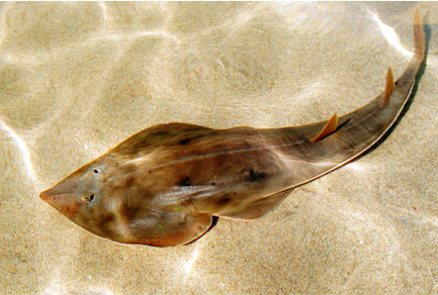
\includegraphics[width=4cm]{images/pezGuitarra.png} }}%
    \qquad
    \subfloat[\centering Imagen de un \textit{dataset} ``complejo'' obtenido de \href{https://www.kaggle.com/c/the-nature-conservancy-fisheries-monitoring}{\textit{The Nature Conservancy}}]{{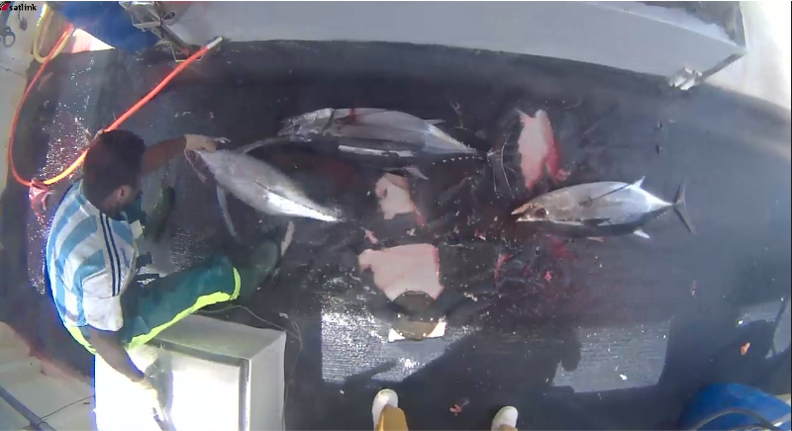
\includegraphics[width=5cm]{images/Bet.png} }}%
    \caption{Comparación de imágenes dentro de datasets diferentes}%
    \label{fig:combined}%
\end{figure}
Además, existen clasificaicones de \textit{datasets}, cada uno con una función de distribución de imágenes y un objetivo específico. En la primera categoría, encontramos conjuntos de datos homogéneos y heterogéneos. Los \textit{datasets} homogéneos se caracterizan por tener la misma cantidad (o un número similar) de muestras por clase, lo que permite que los modelos aprendan de manera equitativa de cada clase. Sin embargo, esto no siempre refleja la realidad, donde la probabilidad de que aparezca una clase de objeto determinada puede ser mayor o menor que otra.
\\\\
En ese sentido, los conjuntos de datos heterogéneos son aquellos que no tienen un número igual de muestras para cada clase. Esto puede ser intencional, ya que el creador del conjunto de datos diseñó la distribución de muestras de esa manera, o puede ser resultado de la falta de muestras disponibles.
\\\\
Además, los \textit{datasets} suelen venir etiquetados en relación a su objetivo. En nuestro caso, para entrenar una CNN, se dispone de un repositorio de imágenes junto con sus etiquetas correspondientes. En cambio, para entrenar una red como YOLO, se requieren los ``bounding boxes'' que delimitan la ubicación de los objetos.
\\\\

Dado que encontrar un \textit{dataset} de este tipo resulta inviable para el caso peruano, se han utilizado dos tipos de conjuntos de datos encontrados en la plataforma Kaggle para esta investigación. Ambos conjuntos contienen imágenes y sus respectivas etiquetas, pero uno presenta peces centrados y sin ruido, mientras que el otro incluye fotografías tomadas en un entorno real donde se encuentran peces, personas e instrumentos de pesca, lo que lo convierte en un conjunto de datos heterogéneo. El primero se utilizará para realizar comparaciones entre los modelos, mientras que el segundo se empleará para el entrenamiento y prueba del pipeline final.
\\\\
Estas imágenes serán re-dimencionadas dependiendo del tamaño de entrada que se espera para cada red, para luego ser pasadas al clasificador.

\section{Detector}
Para la detección de cada imagen del \textit{dataset}, utilizaremos un módulo de detección basado en YOLO v5, el cual ya ha sido preentrenado con el conjunto de datos ``Objects365'', brindando la capacidad de detectar la categoría de peces. Además, se entrenó un YOLO v5 con el \textit{dataset}, ignorando las clases detectadas. Por último, también utilizaremos un modelo llamado UniDet, el cual ha sido entrenado con los \textit{datasets} ``Objects365'', ``OpenImages'' y ``COCO''.  Una vez que las imágenes sean procesadas por el detector, esperamos obtener \textit{los bounding boxes} donde se encuentren los peces individualmente. Se puede visualizar este proceso en la imagen \ref{fig:detector_pez}.
\begin{figure}[h!]
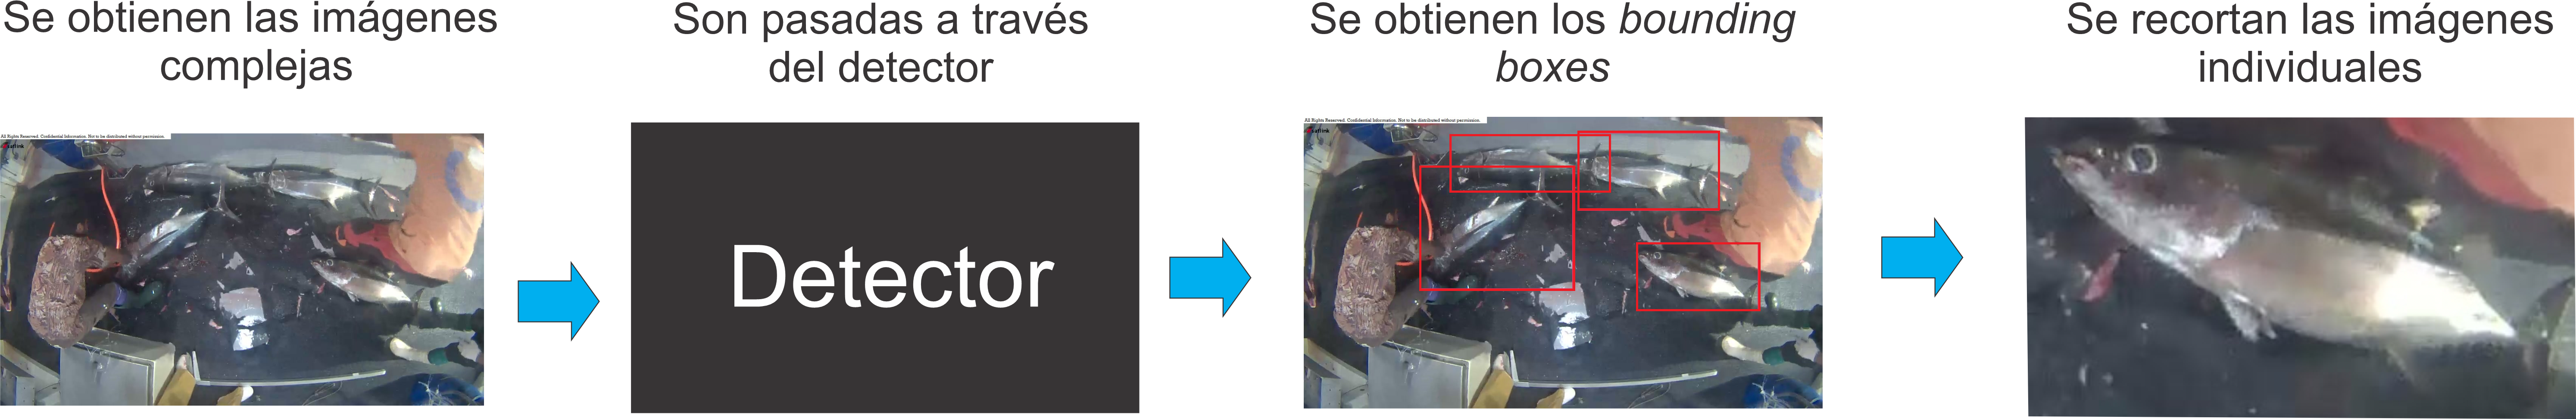
\includegraphics[width=1\textwidth]{images/detector_pez.png}
\caption{Flujo de entrada y salida del detector }
\label{fig:detector_pez}
\end{figure}



\section{Clasificador}
Una vez ubicados los peces, se procede a recortar y redimencionar las imágenes para ocupar la entrada que espera el clasificador. Para los experimentos, se utilizará la resolución específica para cada una de las redes a probar. Cada una de estas redes también serán obtenidas con sus pesos pre-entrenados con ``Imagenet", pero a ellas se les aplicará el proceso de TL, congelando todas las capas convolucionales. Por último, a cada uno de estos modelos se les añadirá una capa llamada ``\textit{GlobalAveragePooling}'' y finalmente ser pasada a las capas clasificadoras. Se espera que con este procedimiento se disminuya el número de parámetros finales que pasarán a la capa de clasificación y mejorar también su precisión y reducirá su tiempo de entrenamiento. El flujo se ve evidenciado en la imagen \ref{fig:clasificador_pez}.
\begin{figure}[h!]
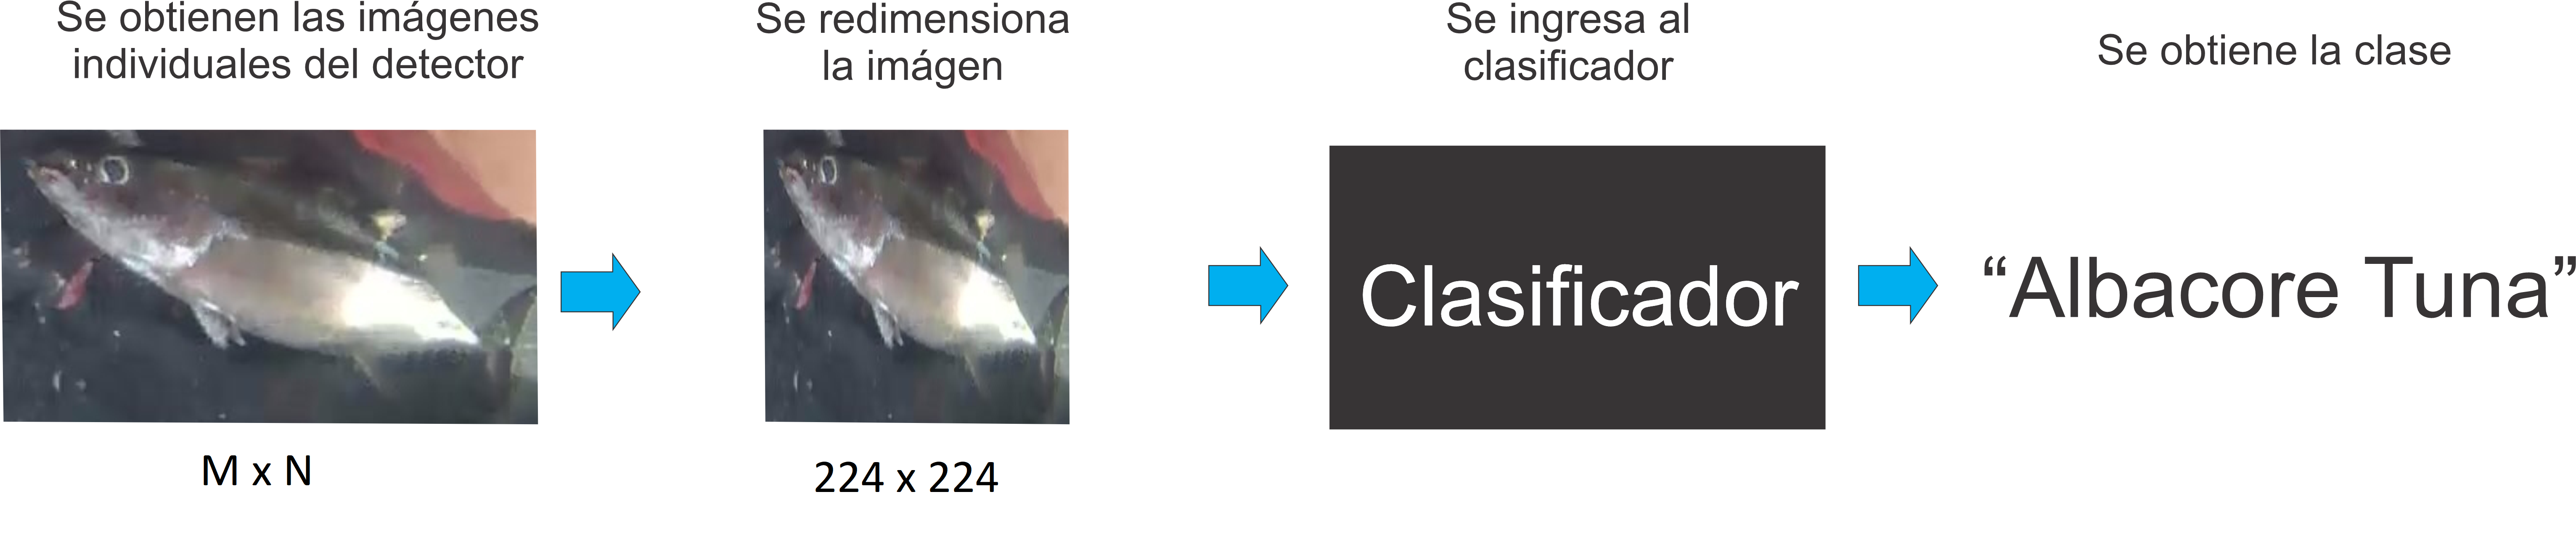
\includegraphics[width=1\textwidth]{images/clasificador_label.png}
\caption{Flujo de entrada y salida del clasificador }
\label{fig:clasificador_pez}
\end{figure}

\section{\textit{Labeled Boxes}}
Después de haber clasificado todas las imágenes de las instancias de peces obtenidas por el detector, se procederán a obtener todas las etiquetas obtenidas, asignándolas a cada uno de los \textit{bounding boxes} que se habían generado anteriormente. En ese sentido se obtendrá como salida la imagen con los \textit{labeled boxes} para cada instancia de pez que se encuentre. 

\section{Evaluación de modelos}

Orhan Yalsin, en 2020 relizó un resumen acerca de algunas métricas que ayudan a comparar algunos de los modelos del estado del arte, de lo cual nos guiaremos para la evaluación de los mismos. Los datos se resumen en la tabla \ref{evaluación}.
\begin{table}[h!]
    \begin{tabular}{|l|r|r|r|r|r|}
    \hline
    \textbf{Model}    & \multicolumn{1}{l|}{\textbf{Size}} & \multicolumn{1}{l|}{\textbf{\begin{tabular}[c]{@{}l@{}}Top-1 \\ Accuracy\end{tabular}}} & \multicolumn{1}{l|}{\textbf{\begin{tabular}[c]{@{}l@{}}Top-5 \\ Accuracy\end{tabular}}} & \multicolumn{1}{l|}{\textbf{Parameters}} & \multicolumn{1}{l|}{\textbf{Depth}} \\ \hline
    Xception          & 88 MB                              & 0.790                                                                                   & 0.945                                                                                   & 22,910,480                               & 126                                 \\ \hline
    VGG16             & 528 MB                             & 0.713                                                                                   & 0.901                                                                                   & 138,357,544                              & 23                                  \\ \hline
    VGG19             & 549 MB                             & 0.713                                                                                   & 0.900                                                                                   & 143,667,240                              & 26                                  \\ \hline
    ResNet50          & 98 MB                              & 0.749                                                                                   & 0.921                                                                                   & 25,636,712                               & -                                   \\ \hline
    ResNet101         & 171 MB                             & 0.764                                                                                   & 0.928                                                                                   & 44,707,176                               & -                                   \\ \hline
    ResNet152         & 232 MB                             & 0.766                                                                                   & 0.931                                                                                   & 60,419,944                               & -                                   \\ \hline
    ResNet50V2        & 98 MB                              & 0.760                                                                                   & 0.930                                                                                   & 25,613,800                               & -                                   \\ \hline
    ResNet101V2       & 171 MB                             & 0.772                                                                                   & 0.938                                                                                   & 44,675,560                               & -                                   \\ \hline
    ResNet152V2       & 232 MB                             & 0.780                                                                                   & 0.942                                                                                   & 60,380,648                               & -                                   \\ \hline
    InceptionV3       & 92 MB                              & 0.779                                                                                   & 0.937                                                                                   & 23,851,784                               & 159                                 \\ \hline
    InceptionResNetV2 & 215 MB                             & 0.803                                                                                   & 0.953                                                                                   & 55,873,736                               & 572                                 \\ \hline
    MobileNet         & 16 MB                              & 0.704                                                                                   & 0.895                                                                                   & 4,253,864                                & 88                                  \\ \hline
    MobileNetV2       & 14 MB                              & 0.713                                                                                   & 0.901                                                                                   & 3,538,984                                & 88                                  \\ \hline
    DenseNet121       & 33 MB                              & 0.750                                                                                   & 0.923                                                                                   & 8,062,504                                & 121                                 \\ \hline
    DenseNet169       & 57 MB                              & 0.762                                                                                   & 0.932                                                                                   & 14,307,880                               & 169                                 \\ \hline
    DenseNet201       & 80 MB                              & 0.773                                                                                   & 0.936                                                                                   & 20,242,984                               & 201                                 \\ \hline
    NASNetMobile      & 23 MB                              & 0.744                                                                                   & 0.919                                                                                   & 5,326,716                                & -                                   \\ \hline
    NASNetLarge       & 343 MB                             & 0.825                                                                                   & 0.960                                                                                   & 88,949,818                               & -                                   \\ \hline
    EfficientNetB0    & 29 MB                              & 0.771                                                                                   & 0.933                                                                                   & 5,330,571                                & -                                   \\ \hline
    EfficientNetB1    & 31 MB                              & 0.791                                                                                   & 0.944                                                                                   & 7,856,239                                & -                                   \\ \hline
    EfficientNetB2    & 36 MB                              & 0.801                                                                                   & 0.949                                                                                   & 9,177,569                                & -                                   \\ \hline
    EfficientNetB3    & 48 MB                              & 0.816                                                                                   & 0.957                                                                                   & 12,320,535                               & -                                   \\ \hline
    EfficientNetB4    & 75 MB                              & 0.829                                                                                   & 0.964                                                                                   & 19,466,823                               & -                                   \\ \hline
    EfficientNetB5    & 118 MB                             & 0.836                                                                                   & 0.967                                                                                   & 30,562,527                               & -                                   \\ \hline
    EfficientNetB6    & 166 MB                             & 0.840                                                                                   & 0.968                                                                                   & 43,265,143                               & -                                   \\ \hline
    EfficientNetB7    & 256 MB                             & 0.843                                                                                   & 0.970                                                                                   & 66,658,687                               & -                                   \\ \hline
    \end{tabular}
    \caption{Evaluación de diferentes modelos. Tabla brindada por Orhan Yalcin \protect\cite{DataModelos}. }
    \label{evaluación}
\end{table}

%\begin{figure}[h!]
%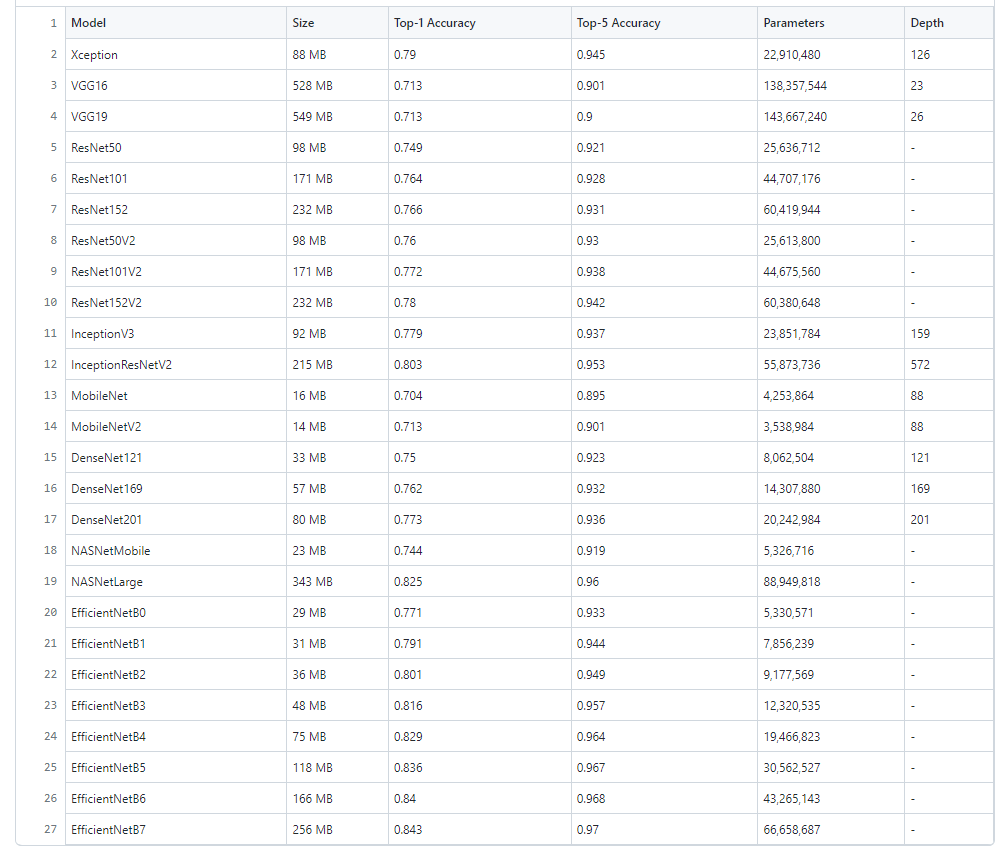
\includegraphics[width=1.3\textwidth]{images/EvaluacionModelos.png}
%\caption{Evaluación de diferentes modelos. Tabla brindada por Orhan Yalcin \cite{DataModelos}. }
%\label{evaluación}
%\end{figure}

Dentro de esta tabla se pueden resaltar varios modelos interesantes: VGG19 (si consideramos solo las capas convolucionales), ResNet50, InceptionV3, y los EfficientNetBX resultan tener una buena relación entre el peso, el número de parámetros y la precisión que estas obtienen, esta última siendo de las más altas dentro de todos estos modelos. Se tendrá en consideración que este pipeline planea ser ejecutado en vídeos en tiempo real y por ello se necesita que el modelo sea el más pequeño posible evitando perder la precisión. Por otra parte, están las MobileNet, ya han sido utilizadas para el procesamiento de imágenes en tiempo real por ser más ligeras, enfocadas a ser utilizadas en celulares. Creemos que todas estas redes son aptas para este problema y pasarán a ser evaluadas en el siguiente capítulo, en base al primer \textit{dataset} mencionado anteriormente. \\\\
Una vez analizado esas redes en base al \textit{dataset}, se compararán la precisión y costo entre ellas y se obtendrá la que finalmente pasará a formar parte del \textit{pipeline} final, en donde será encargada de clasificar cada imagen obtenida por la red Yolo.\\\\
En el siguiente capítulo finalmente se verá la experimentación con todos los modelos anteriormente señalados, tanto como la especificación de las imágenes y la experimentación del \textit{pipeline} final.